% Assignment 3 report on PATRA, in the ICML template.
% Numbers are checked against ../results by check_numbers.py.
\documentclass{article}

\usepackage[T1]{fontenc}
\usepackage{microtype}
\usepackage{graphicx}
\usepackage{booktabs}
\usepackage{hyperref}
\usepackage[accepted]{icml2025}
\usepackage{amsmath}
\usepackage{xcolor}
\newcommand{\minh}[1]{\textcolor{red}{[Minh: #1]}}
\hypersetup{pdfsubject={Assignment 3 report}}
\icmltitlerunning{A Self-Study of PATRA}
\renewcommand{\bibfont}{\fontsize{7.5}{8.5}\selectfont}
\setlength{\bibsep}{0.5pt}
\setlength{\intextsep}{4pt plus 1pt minus 1pt}
\setlength{\textfloatsep}{8pt plus 2pt minus 2pt}
\makeatletter
\def\section{\@startsection{section}{1}{\z@}{-0.08in}{0.01in}{\large\bf\raggedright}}
\makeatother

\begin{document}

\twocolumn[
\icmltitle{PATRA: Reproduction, Insights, and Proposal}

\vskip -0.12in
\begin{icmlauthorlist}
\icmlauthor{Minh Tran}{}
\end{icmlauthorlist}
\vskip 0.3in
\icmlkeywords{Time Series Question Answering, Reproducibility}
]

\begin{abstract}
Time Series Question Answering (TSQA) has emerged rapidly as sequential data becomes increasingly prevalent across various domains. Current approaches enable LLMs to answer questions and reason about trends and conclusions drawn from numerical data. However, existing methods often treat time series values as plain text or attach series embeddings to prompts, struggling to connect questions with temporal patterns such as trends and seasonality. PATRA addresses these challenges through pattern-aware alignment and a task-balanced reward mechanism. In this report, I investigate the published model and dataset, run intervention experiments to test whether the model actually understands the time series, and discuss the paper's strengths and limitations, proposed improvements and my reflections. Code and results are available at \href{https://github.com/coutMinh/Timeseries-Study}{\textcolor{magenta}{\texttt{code}}}.
\end{abstract}


\section{Introduction}

PATRA \citep{lu2026patra} identified two key limitations in existing TSQA approaches \citep{kong2025timemqa}: weak grounding in temporal patterns and the dominance of easier tasks during training. By introducing latent trend and seasonal alignment alongside reinforcement learning with a balanced reward mechanism, PATRA achieved the best results among open-source models across all eight evaluation metrics.

\section{Related Work}

\emph{(i) TSQA.}
\emph{Time-MQA} \citep{kong2025timemqa} lets users ask natural-language questions about time series, covering numerical analysis and open-ended reasoning.
\emph{(ii) LLMs and multimodal LLMs for time series.}
\emph{TimeOmni-1} \citep{guan2026timeomni} and \emph{Time-R1}~\cite{liu2025timer1} feed values to the LLM as text, while \emph{ChatTS} \citep{xie2025chatts} and \emph{IT-Former} \citep{wang2025itformer} treat the series as a separate modality. Recent work has used RL to improve LLMs' temporal reasoning~\citep{liu2025timer1}, including reasoning over numerical time series~\citep{guan2026timeomni}.
\emph{(iii) Do LLMs actually read the series?}
To look inside these models, I asked one main question while reading these works: do they actually read the series? High scores alone cannot show this. For example, in NLI tasks, models predict from the hypothesis without reading the premise \citep{gururangan2018annotation}, and TSQA models could likewise answer from the question alone. For TSQA, \citet{chen2026evidence} alter the input series of four systems, and find that aggregate scores can hide how the numbers are used.

\begin{figure}[!t]
\vskip -0.1in
\centering
\includegraphics[width=1\columnwidth]{figures/robot_thumbnail.pdf}
\vskip -0.05in
\caption{TSQA problems.}
\label{fig:thumbnail}
\end{figure}

\section{Self-Study of the Published Model}

\textbf{Reproduction.}
I ran inference based on the published weight and dataset of the original paper PATRA. Table~\ref{tab:repro} shows ROUGE-L close to the paper and accuracy 10.19--25.86 points below it. Four prompt and generation variants reach at most 52.05\%.

\begin{table}[H]
\caption{Re-run of the published PATRA-7B, with paper values in parentheses.}
\label{tab:repro}
\vskip 0.05in
\centering
\small
\begin{tabular}{lrcc}
\toprule
Task & $n$ & Accuracy (\%) & ROUGE-L \\
\midrule
Comprehension & 116 & 30.17 (56.03) & 27.39 (25.67) \\
Recognition & 725 & 54.07 (64.69) & 26.02 (25.46) \\
Reasoning & 148 & 32.43 (44.59) & 29.04 (27.36) \\
Prescience & 108 & 42.59 (52.78) & 27.55 (27.06) \\
\bottomrule
\end{tabular}
\vskip -0.1in
\end{table}


\textbf{Self-study ablation.}
Inspired by \citet{chen2026evidence}, I test how changes to the
time-series input and processing affect PATRA at inference.
Across the three interventions, accuracy ranges from 47.95\% to 48.77\%,
compared with 47.49\% in the unmodified run (Table~\ref{tab:ablation}).
Replacing the series with zeros changes 3.28\% of answers.
In separate tests, changing the prompt template changes 18.41--25.43\%
of answers.

\begin{table}[!t]
\caption{Accuracy on the 1,097 labeled questions under interventions.}
\label{tab:ablation}
\vskip 0.05in
\centering
\small
\begin{tabular*}{\columnwidth}{@{\extracolsep{\fill}}lr@{}}
\toprule
Condition & Acc.\ (\%) \\
\midrule
Unmodified & 47.49 \\ 
Series replaced by zeros & 48.13 \\
Random encoder and alignment & 48.77 \\
Alignment bypassed & 47.95 \\
\bottomrule
\end{tabular*}
\vskip -0.1in
\end{table}


\textbf{Implementation insights.} I summarized insights as follow.

\emph{(1) The decomposition can keep trend and seasonality.}
PATRA packs every 16 points into one token and splits the tokens into a long-term direction (trend) and repeating cycles (seasonality) with a moving average.
In the paper case studies, the latent trend correlates 0.986 with the true trend and the latent seasonality 0.938 with the true cycle.

\emph{(2) The evaluation series are too short for this split.}
The moving average spans 25 tokens but evaluation series have at most 30 points, so one or two tokens, and the split reduces to their mean and difference. Section~5.10 does not state the length of its synthetic series.

\emph{(3) The model cannot see the numbers it is asked to quote.}
The code normalizes each series and do not include offset and scale to the prompt, but there are 77.02\% of numbers in the training need raw values in the answers.

\emph{(4) My core question: text or embeddings?}
\emph{TimeOmni-1} and \emph{Time-MQA} put the numerical sequence into the prompt as text, while \emph{PATRA} and \emph{ChatTS} turn it into embeddings with a dedicated encoder. I wondered whether text makes exact values easier to read and how the LLM learns to interpret an encoder's embeddings.
The released models suggest an answer. On open-ended questions, 94.25\% of the numbers Qwen quotes occur in the raw series, against 3.44\% for PATRA. Interestingly, some of the numbers PATRA quotes do not appear in any related series. Inside PATRA, the alignment attention is nearly uniform: replacing it with a plain average changes its output by only 0.005\%.

\section{Strengths and Limitations}

\textbf{Strengths.} The paper identifies two concrete challenges in time-series question answering and uses targeted ablations to evaluate the contribution of each proposed component. 

\textbf{Limitations.}

\emph{(i) Limited access to the original series.}
PATRA encodes each 16-point patch as one token. It fuses these tokens with the question once, before generating an answer. If the LLM needs to verify a peak or quote an exact value during generation, it can attend to the fused tokens but has no way to retrieve the original observations. 

\emph{(ii) Highly volatile, non-stationary sequences:} On the 287 most volatile evaluation series (top 10\% by spread-normalized point-to-point changes), PATRA correctly answers only 5 of 21 trend questions. As illustrated in Figure~\ref{fig:failure}, five representative failures exhibit repetitive reasoning patterns and unsupported numerical claims, with quoted values absent from both the raw and normalized series.

\begin{figure*}[!t]
\centering
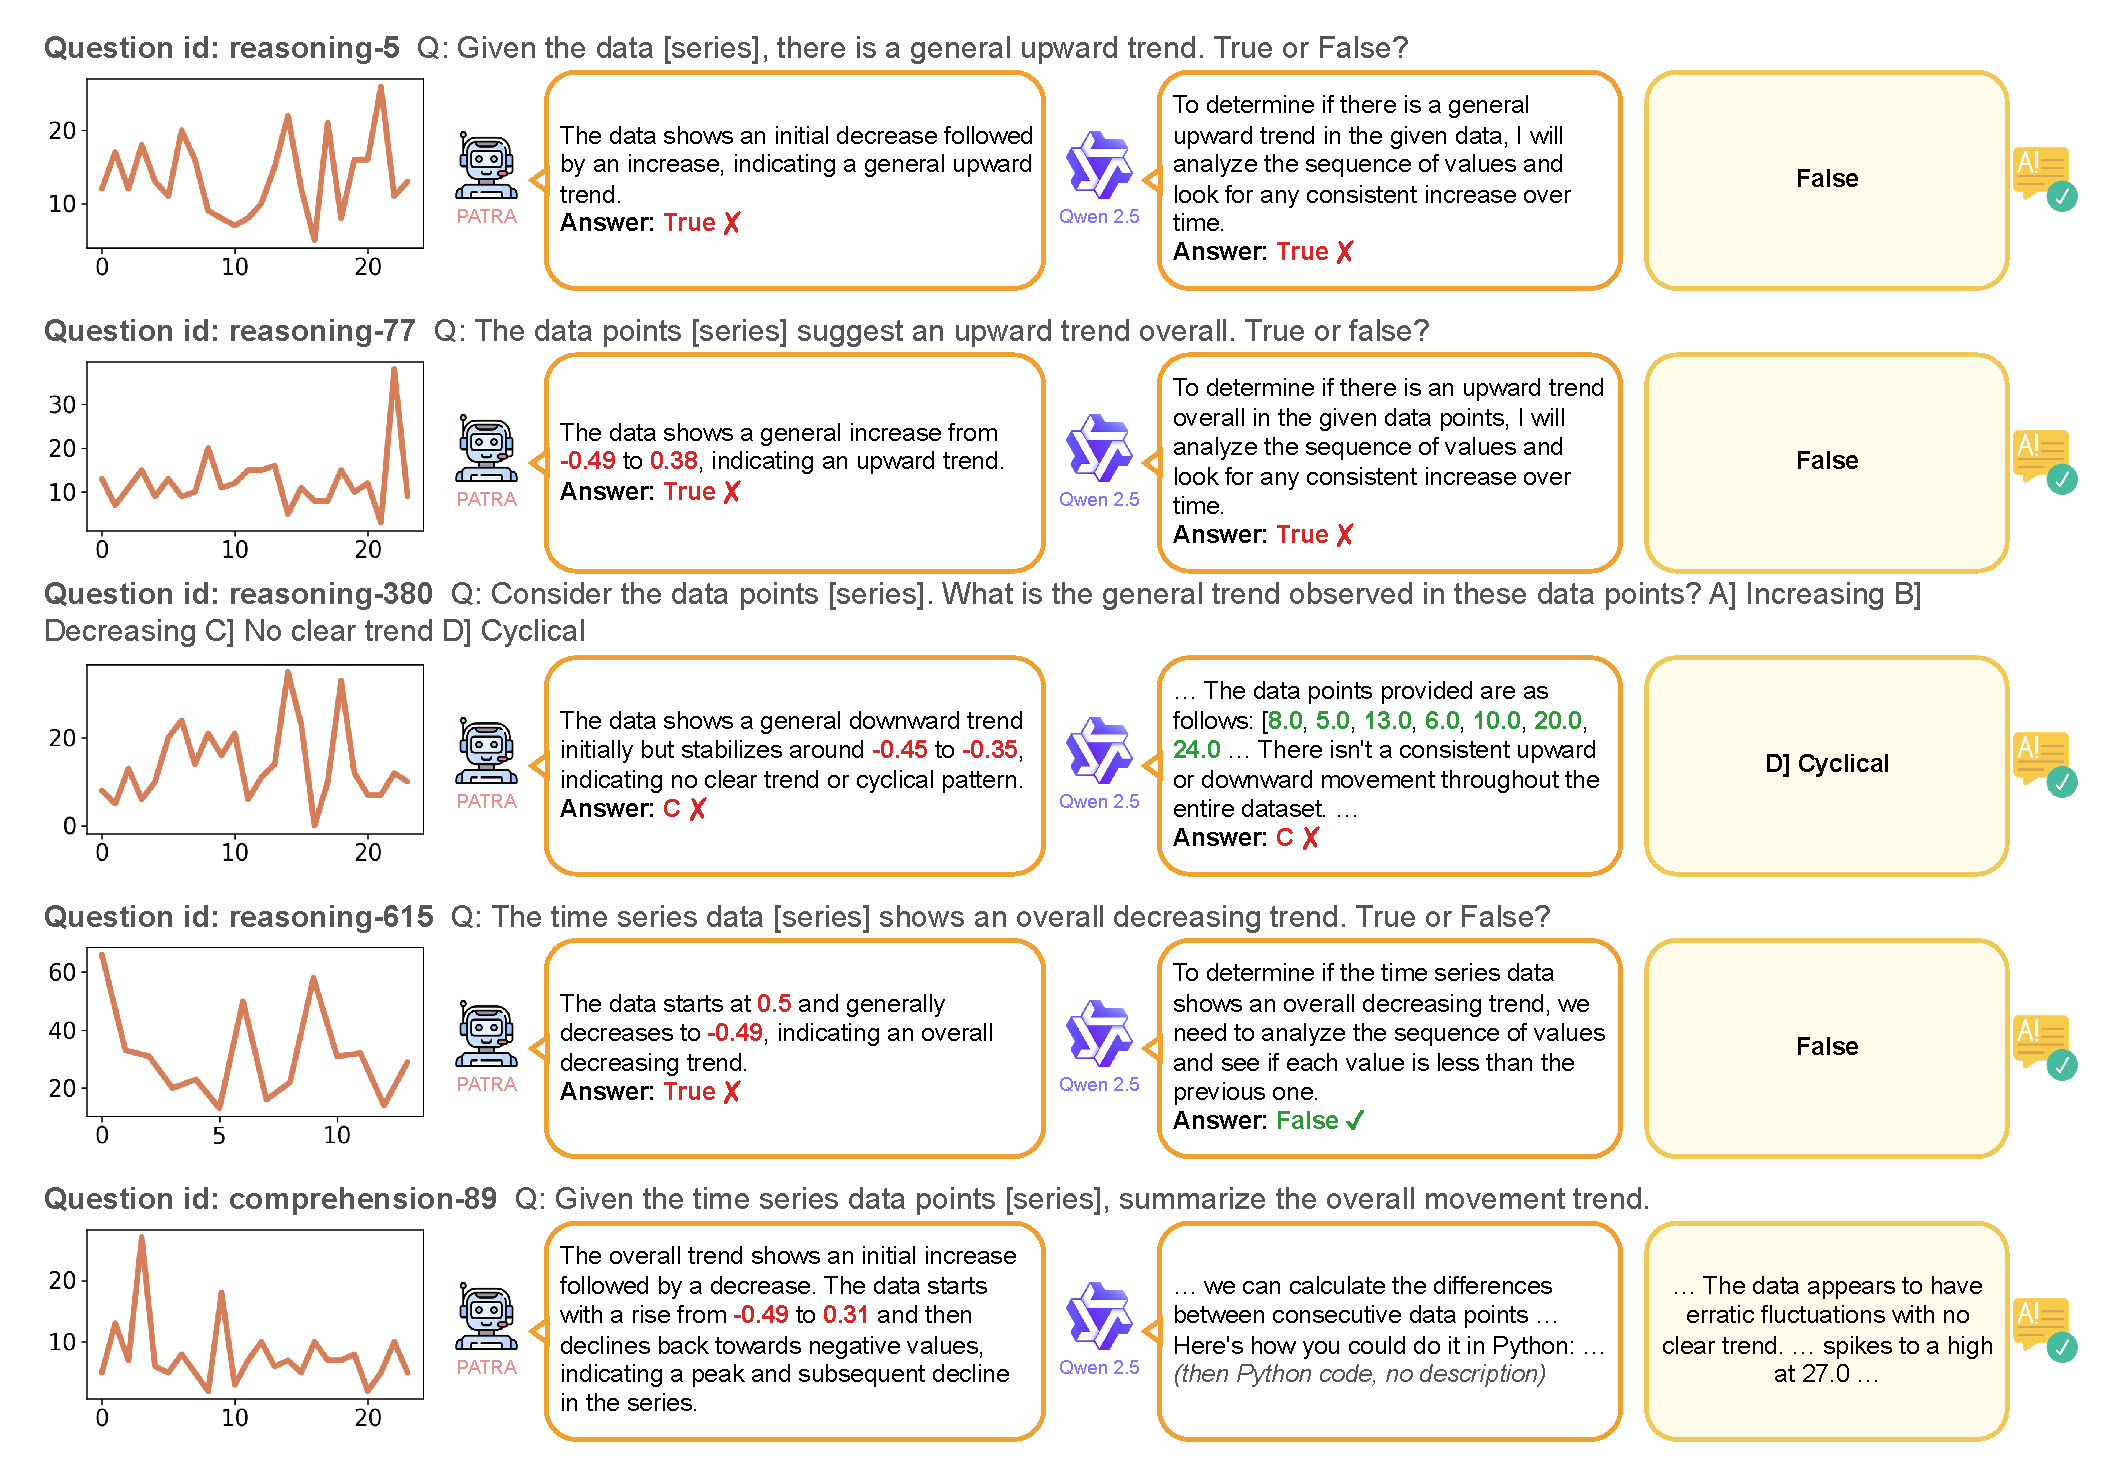
\includegraphics[width=\textwidth]{figures/failure_decomposition.pdf}
\vskip -0.1in
\caption{Five trend-analysis failures of the released PATRA-7B on volatile time series, alongside Qwen2.5-7B responses and reference answers. Green values match observed points, while red values are absent from both the raw and normalized series.}
\label{fig:failure}
\end{figure*}


\textbf{Proposals.} I propose Tool-Augmented Time-Series Reasoning, extending PATRA with an external numerical tool interface. During autoregressive generation, the LLM can invoke tools to retrieve exact observations or compute temporal statistics (e.g., local trends, extrema, and segment differences). The tool results are returned as textual evidence to the LLM, enabling it to verify numerical claims and refine its reasoning without reconstructing values from compressed embeddings. This requires modifying the decoding workflow and optionally fine-tuning the LLM for tool use, rather than retraining the entire encoder.

\section{Research Direction and Reflection}

I have gained a lot of new knowledge while exploring these research directions. After reviewing several previous works on TSQA, including text-based approaches~\cite{kong2025timemqa}, fusion-based approaches~\cite{lu2026patra}, and reasoning-enhanced time series models~\cite{guan2026timeomni}, I came across a recent survey~\cite{anonymous2026the} that introduces an emerging research direction: applying agentic systems to time series tasks which align the most with \textbf{FPT research direction}. The survey identifies six main research frontiers: (i) Verifiable Temporal Reasoning, (ii) End-to-End Agentic Training, (iii) Memory and Lifelong Adaptation, (iv) Temporal World Models, (v) Decision-Centric Evaluation, and (vi) Standardized Temporal Tooling. These research directions could address several limitations of current time-series reasoning systems, including weak grounding in numerical data, difficulty combining evidence across time windows, unreliable multi-step reasoning, evaluation metrics that miss intermediate errors, and limited adaptation to new events. The direction that inspires me most is memory and lifelong adaptation for time-series agents. This is a critical research question in an era of rapid change across economics, technology, AI, and military affairs.

\bibliography{references}
\bibliographystyle{icml2025}

\end{document}
